\documentclass{article}
\usepackage[utf8]{inputenc}
\usepackage{titling}
\usepackage{graphicx}
\usepackage[colorlinks=true,linkcolor=blue]{hyperref}
\usepackage[spanish]{babel}


\title{Criptografía clásica}
\author{Cristina Díaz García}
\date{October 2018}

\renewcommand\maketitlehooka{\null\mbox{}\vfill}
\renewcommand\maketitlehookd{\vfill\null}


\begin{document}

\addcontentsline{toc}{section}{Índice general}

\begin{titlingpage}
\maketitle
\end{titlingpage}

\newpage

\tableofcontents

\newpage

\section{Ejercicio 1}
\subsection{Apartado a}
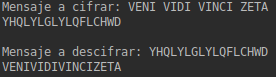
\includegraphics[scale=0.7]{1a.png} 

\subsection{Apartado b}
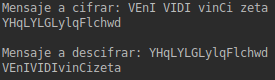
\includegraphics[scale=0.7]{1b.png}

\subsection{Apartado c}
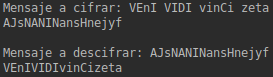
\includegraphics[scale=0.7]{1c.png}

\newpage

\section{Ejercicio 2}
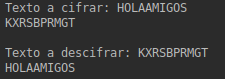
\includegraphics[scale=0.7]{2.png}

\end{document}